% ============================================================================================================
% Abraham's contribution, part C: a new section for the written report (place it after "Results").
% Written at the level of ISLP plus three small additions (clusters, the variance of a sample drawn without
% replacement, and a first-order approximation). Formal statements and proofs of the harder results are in
% abraham_appendix_theory.tex. Every number comes from results/*.csv; figures are in report/figures/.
% Theory: proposals/06; draft note proposals/08; adversarial review proposals/09. Pre-registration: PREREG.md.
% ============================================================================================================

\section{How Much Should We Trust a Cross-Validated Number?}
\label{sec:errorbars}

Every number in Section~5 is a cross-validated estimate, and each needs an error bar. The textbook's error bars treat
the observations as independent \cite[Section 5.1.3, pp.~206--208]{James:2023}. Ours are not: a participant appears in up
to 22 dyads, and all dyads in an event share an evening. This section asks three questions: what does
cross-validation estimate when rows come in clusters, which error bars are trustworthy, and does the usual
cross-validated AUC need a correction? Each answer is a short mathematical result, and each prediction was tested on
simulated data, pre-registered before the simulation ran.

\subsection{Setup}

There are $G=21$ events and $n=4{,}184$ dyads. For each dyad $i$ a model makes an error $\ell_i$ (here, $\ell_i=1$ for a wrong
match prediction and 0 otherwise). In event-grouped $K$-fold cross-validation (Section~\ref{sec:beyond}) the events are
dealt into $K$ folds; the model fitted without fold $k$ predicts the dyads in fold $k$, and the cross-validation estimate
is the average error over all dyads,
\[
\widehat{\mathrm{Err}}_{\mathrm{CV}}=\frac1n\sum_{i=1}^n\ell_i .
\]
What a matchmaker wants to know is $\mathrm{Err}_{\mathrm{new}}$, the error rate of the model fitted to all our data when it is
used at a new event, with new people. We call a 90\% interval \emph{trustworthy} if it contains $\mathrm{Err}_{\mathrm{new}}$ about
90\% of the time when the whole study is repeated.

\subsection{What cross-validation estimates}

\begin{lem}\label{lem:what}
Suppose events are drawn independently from the same population. With event-grouped folds, each held-out dyad is,
from the point of view of the model that predicts it, a dyad from a new event, so $\widehat{\mathrm{Err}}_{\mathrm{CV}}$ estimates the
new-event error of a model trained on $(K-1)/K$ of the events. With randomly assigned rows, a held-out dyad's event
(and usually its people) also appear in the training data, so cross-validation estimates the error on events the
model has already seen.
\end{lem}

\begin{proof}
With event-grouped folds, the event of a held-out dyad contributes no rows to the training data, so the dyad is
independent of the fitted model and has the same distribution as a dyad from a new event; its expected error is
therefore the model's new-event error, and averaging over dyads and folds gives the claim. With random rows this
independence fails, because the dyad's event, and its participants, are in the training data.
\end{proof}

This matters in practice. With random rows every model's AUC rises, by 0.08 to 0.13 on the \texttt{pre} features
and by 0.02 to 0.07 on \texttt{pre+date} (Figure~\ref{fig:leakage}): the model partly recognizes people it met in
training. Holding out whole groups is the standard advice for clustered data \cite[pp.~917, 919]{Roberts:2017}.

\begin{figure}[h]
\centering
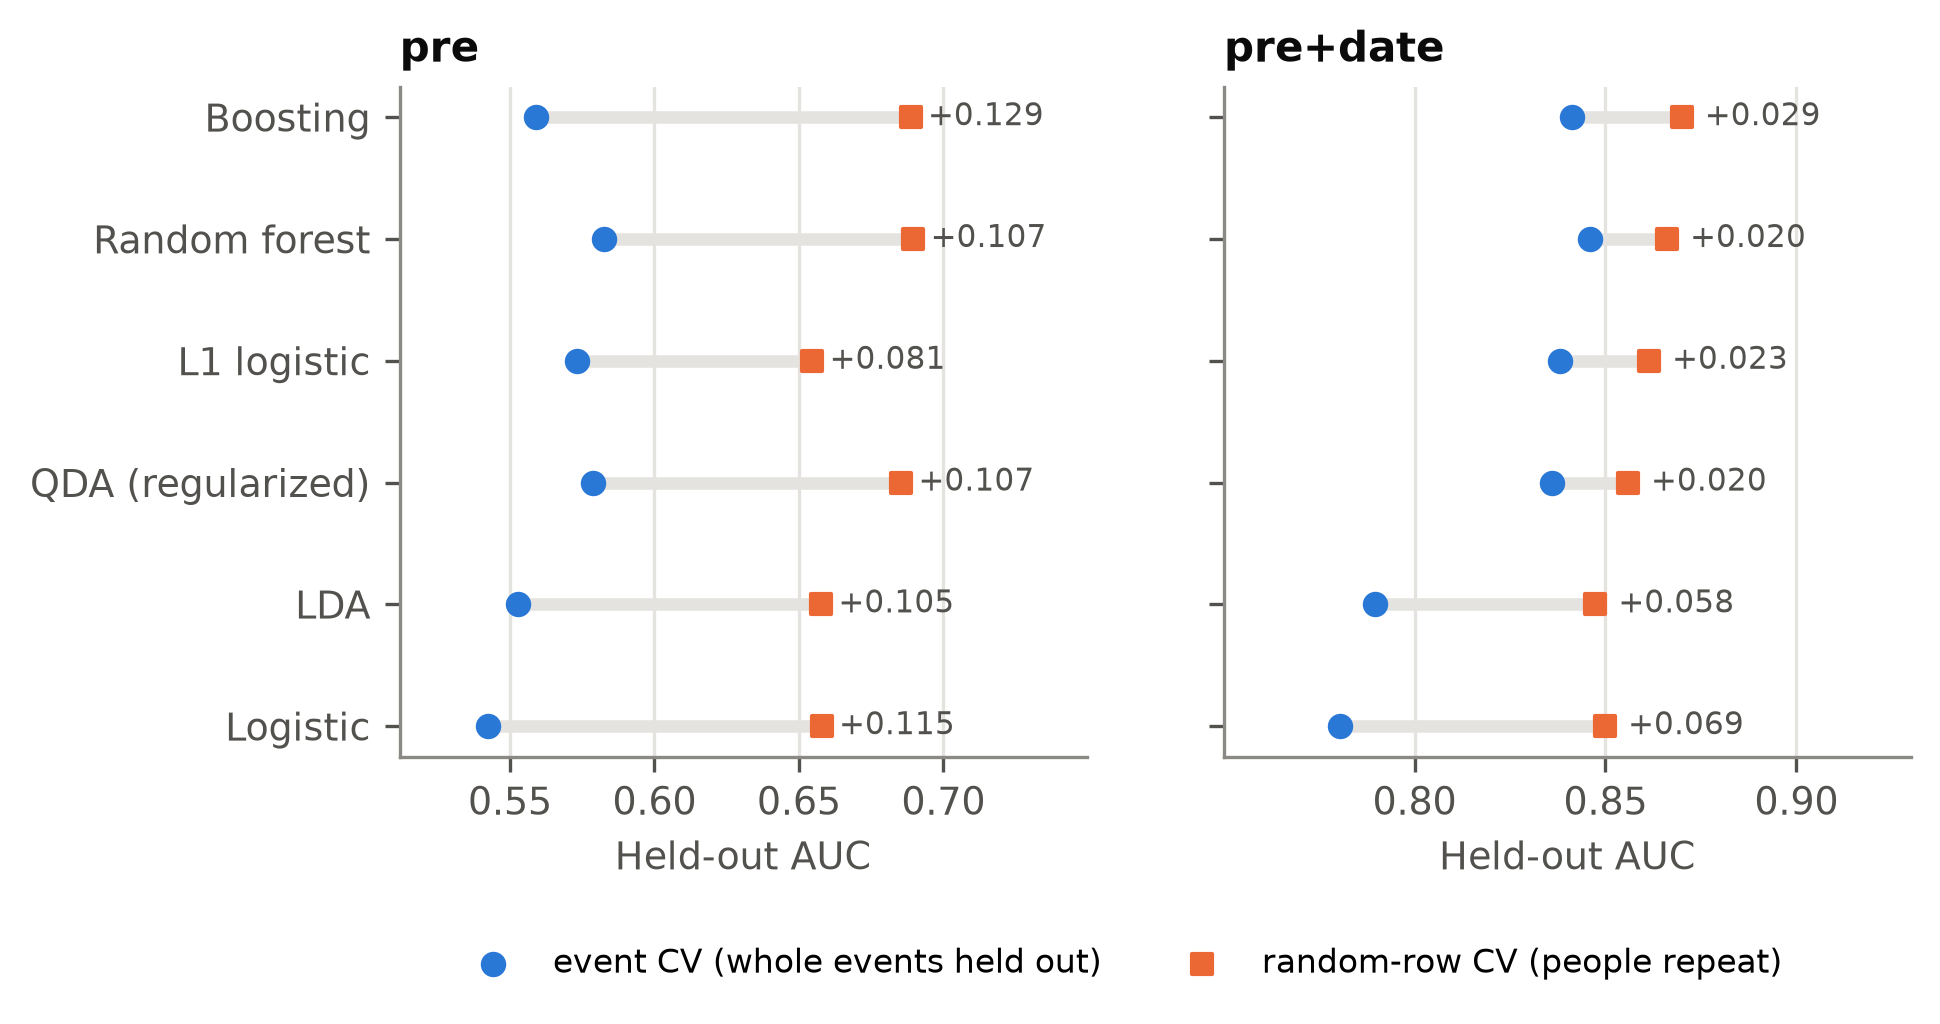
\includegraphics[width=\textwidth]{figures/paper_leakage.png}
\caption{Letting the same people appear in training and test inflates every model's AUC. Held-out AUC under event and
random-row 5-fold cross-validation, same models and features (results/part2\_models\_metrics.csv).}
\label{fig:leakage}
\end{figure}

\subsection{Three error bars}

We compare three ways of putting an error bar on $\widehat{\mathrm{Err}}_{\mathrm{CV}}$ (Section~\ref{sec:beyond}).
\begin{itemize}
\item \emph{Rows independent:} the usual standard error $s/\sqrt n$, where $s$ is the standard deviation of the $\ell_i$.
\item \emph{Cluster-robust:} errors are added up within each event first,
\begin{equation}\label{eq:vcr}
\widehat{\mathrm{SE}}_{\mathrm{CR}}^2=\frac{G}{G-1}\cdot\frac{1}{n^2}\sum_{g=1}^{G}\Big(\sum_{i\in\text{event }g}(\ell_i-\bar\ell)\Big)^2,
\end{equation}
used with $t$ quantiles on $G-1$ degrees of freedom.
\item \emph{Repeated cross-validation (Nadeau--Bengio):} repeat $K$-fold cross-validation $R$ times, giving $J=RK$ fold
errors with sample variance $S^2$, and use the variance $\big(\frac1J+\frac1{K-1}\big)S^2$ \cite[Section 3.1, p.~248]{Nadeau:2003}.
\end{itemize}

\subsection{Result 1: the Nadeau--Bengio correction works only with grouped folds}

\begin{prop}\label{prop:nb}
Hold the dyads' errors fixed, in $G=Kq$ events of equal size, and average the Nadeau--Bengio variance over the random
choice of folds. If the folds are made of whole events, the average is
\[
\frac{J+K-1}{J-1}\times\widehat{\mathrm{SE}}_{\mathrm{CR}}^2 ;
\]
if the folds are random rows, it is the same factor times the rows-independent variance $s^2/n$.
\end{prop}

\begin{proof}
Let $\bar c_g$ be event $g$'s average error and $s_c^2=\frac1{G-1}\sum_g(\bar c_g-\bar\ell)^2$; with equal event sizes,
$\widehat{\mathrm{SE}}_{\mathrm{CR}}^2=s_c^2/G$. The folds of any partition together contain every dyad once, so the $J$ fold errors
average exactly to $\bar\ell$, and the expected sample variance is $E[S^2]=\frac{J}{J-1}\operatorname{Var}(e)$, where $\operatorname{Var}(e)$ is the variance of
one fold's error over the random choice of fold. A grouped fold's error is the average of $q$ event averages drawn
without replacement from the $G$ events, so by the standard formula for sampling without replacement
\cite[Chapter 2]{Wolter:2007},
\[
\operatorname{Var}(e)=\Big(1-\frac qG\Big)\frac{s_c^2}{q}=(K-1)\frac{s_c^2}{G}.
\]
Multiplying $E[S^2]$ by $\frac1J+\frac1{K-1}=\frac{J+K-1}{J(K-1)}$ gives the result. For random rows, replace event
averages by single dyads.
\end{proof}

The factor $(J+K-1)/(J-1)$ is close to 1 when $J$ is large. So the correction measures the cluster-robust spread when the
folds are made of whole events, but only the rows-independent spread when the folds are random rows, and then it is
too small for the same reason the usual standard error is.

\subsection{Result 2: why the cluster-robust error bar is right, and how cautious Nadeau--Bengio is}

A fold's error has two parts. The first is how hard its held-out events happen to be. The second is a small shift
caused by \emph{which} events trained the model: leaving out an easy event makes the model slightly worse, leaving out a
hard one slightly better. Approximating each fitted model to first order around the model a very large study would
fit (a Taylor approximation; Appendix~\ref{app:theory}), the second parts have a useful property: averaged over the $K$
folds they equal the same shift in the final model fitted to all events. They therefore cancel in
$\widehat{\mathrm{Err}}_{\mathrm{CV}}-\mathrm{Err}_{\mathrm{new}}$, so the error of the cross-validation estimate comes from the difficulty of the
held-out events, which is exactly what the cluster-robust standard error measures. The second parts do \emph{not}
cancel in the spread of the fold errors, so the Nadeau--Bengio variance is inflated by a factor that can be computed
from the two parts' variances and their correlation. For the error rate this factor is about 1.2 with five folds; for
the log-likelihood loss the model was fitted with, the shifts vanish and the factor is exactly 1
(Proposition~\ref{prop:first-formal} in Appendix~\ref{app:theory}).

\subsection{Testing the results on simulated data}

Following \cite[Sections 3--5]{Morris:2019}, we simulated many data sets that look like ours, with a known truth, and
counted how often each 90\% interval contained $\mathrm{Err}_{\mathrm{new}}$. The truth is a logistic model fitted to our data, with
extra random effects for each woman, each man and each event; each simulated study draws new events (10, 21 or 40),
new people and new outcomes, and $\mathrm{Err}_{\mathrm{new}}$ is measured on 2,000 further new events. We also used a simpler
balanced design with 20 to 320 clusters to check the large-sample results. Each design used 300 to 400 simulated
studies, so a coverage near 90\% is accurate to about $\pm1.5$ points \cite[Section 5.2, Table 6]{Morris:2019}.

\begin{figure}[h]
\centering
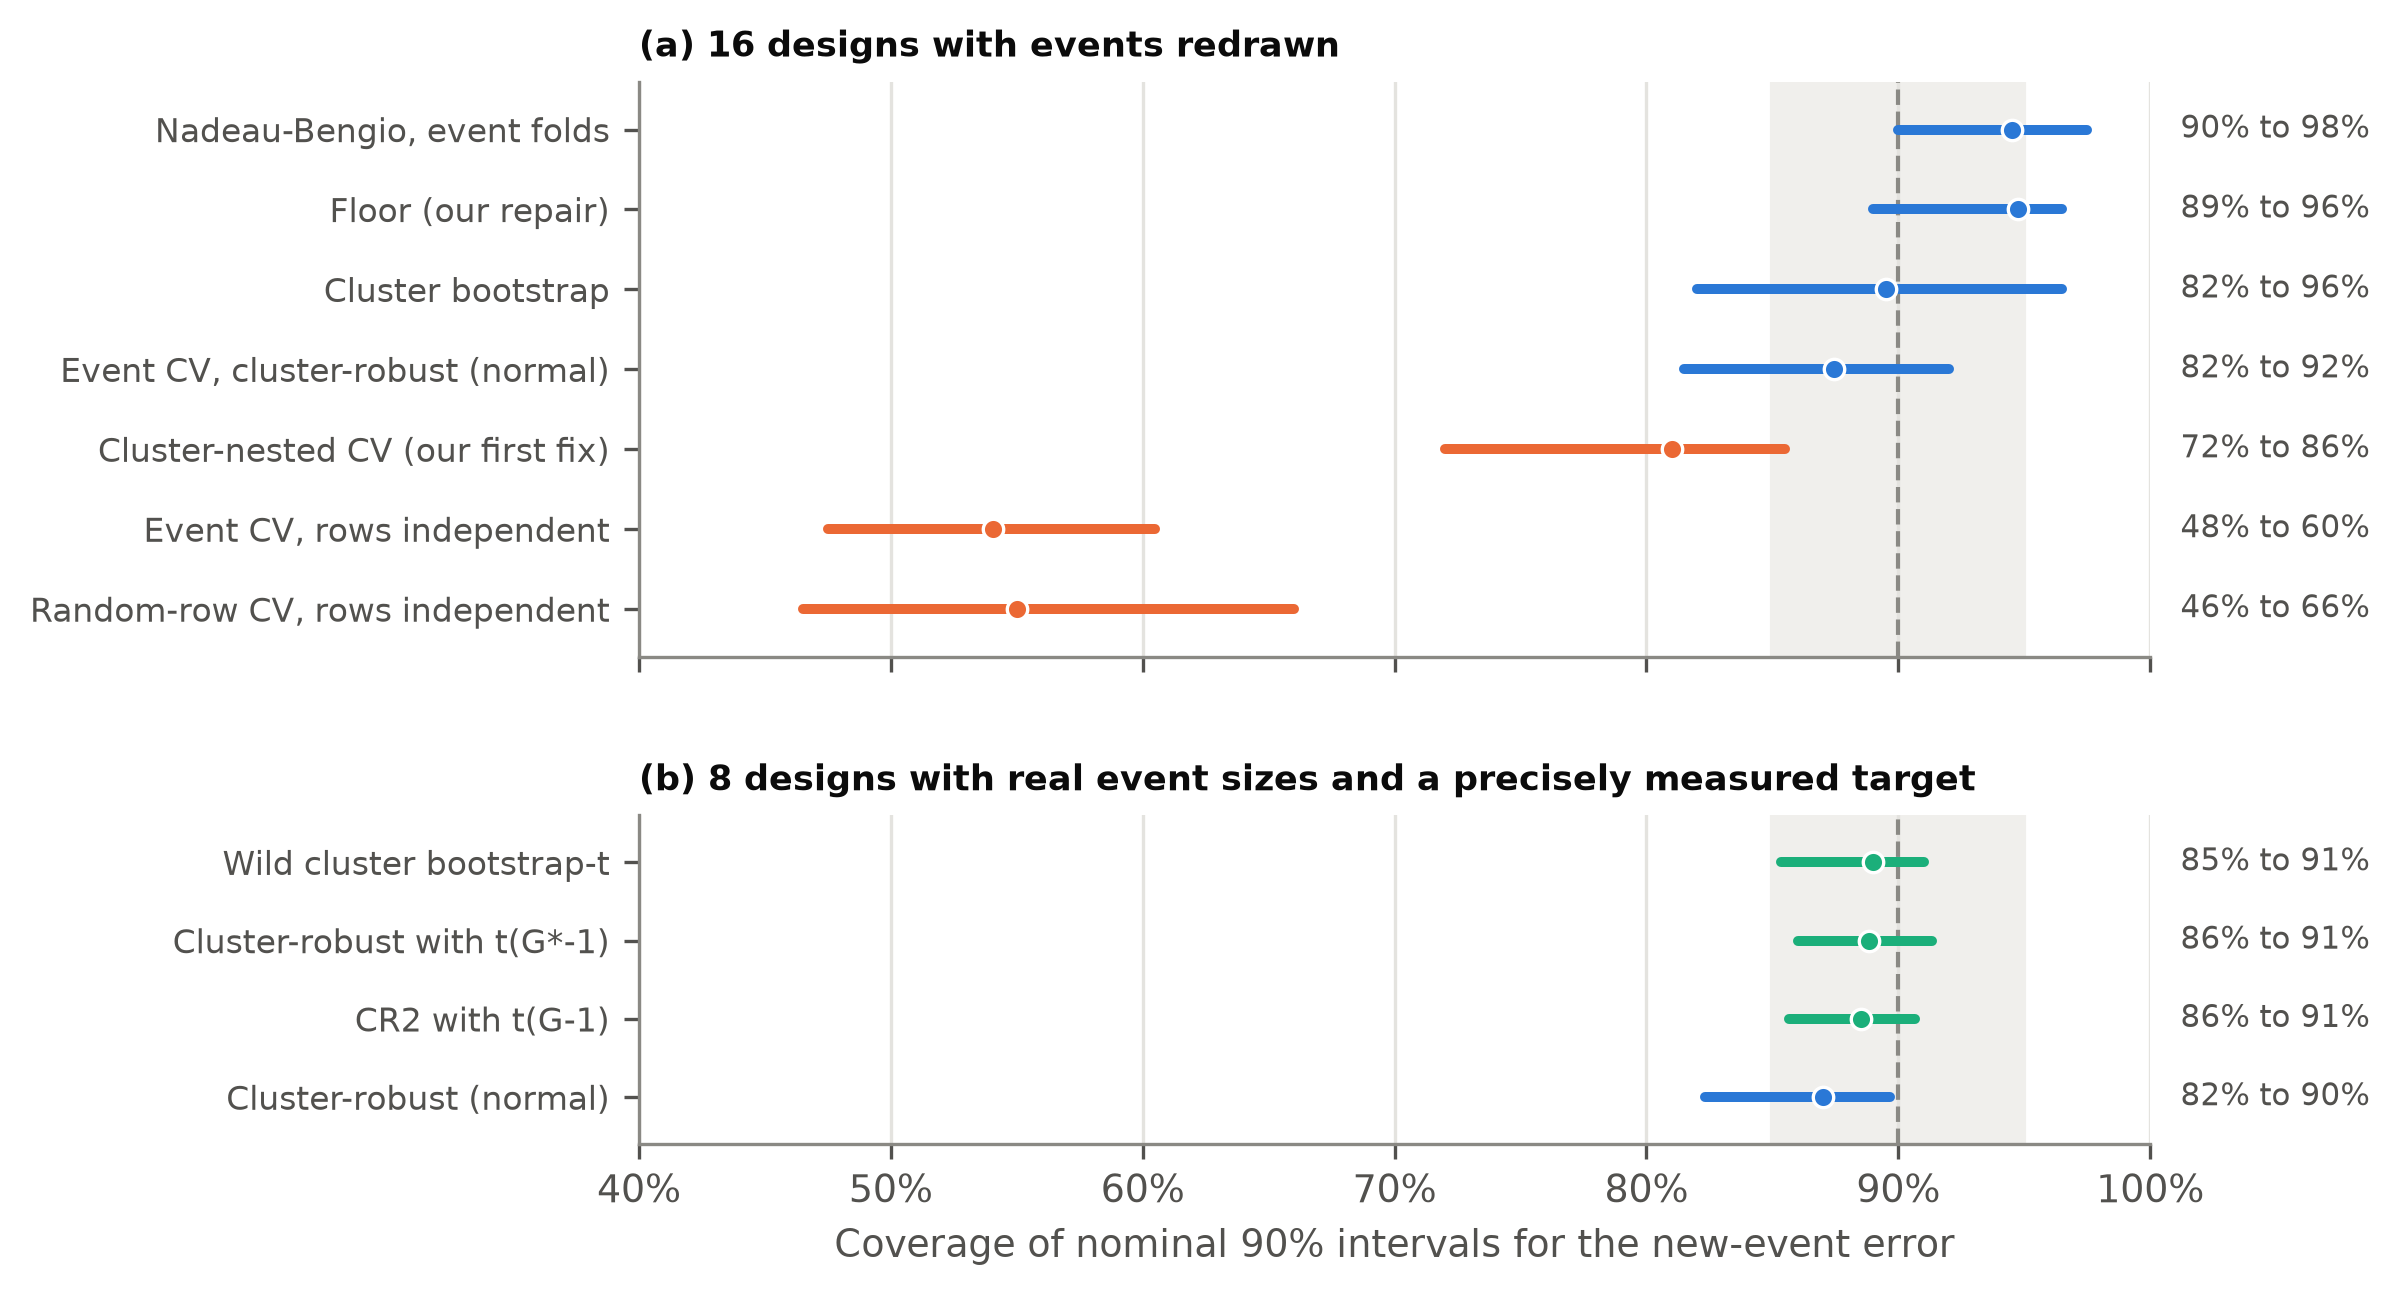
\includegraphics[width=\textwidth]{figures/paper_coverage.png}
\caption{Only event-aware error bars reach their 90\% target. Coverage of nominal 90\% intervals for $\mathrm{Err}_{\mathrm{new}}$:
line, range over designs; dot, median; shaded band, 85\% to 95\%. (a) 16 designs with events redrawn; (b) 8 designs
with the real event sizes and a precisely measured target (results/sim\_cv\_repair\_coverage.csv, sim\_cv\_sizes\_coverage.csv).}
\label{fig:coverage}
\end{figure}

\emph{Which error bars are trustworthy} (Figure~\ref{fig:coverage}). Intervals that treat rows as independent covered
46\% to 66\% of the time, roughly half. Our first proposal, an event-grouped version of the nested cross-validation
of Bates, Hastie and Tibshirani \cite[Section 4]{Bates:2024}, covered only 72\% to 86\%, and we report it as a failure.
Event-aware intervals reached their target: the cluster-robust interval with $t$ quantiles covered 86\% to 91\%, the
wild cluster bootstrap 85\% to 91\%, and the Nadeau--Bengio correction on event folds 90\% to 98\% (slightly cautious, as
Result~2 predicts). On random-row folds the same correction covered only 52\% to 76\%, as Result~1 predicts.

\begin{figure}[h]
\centering
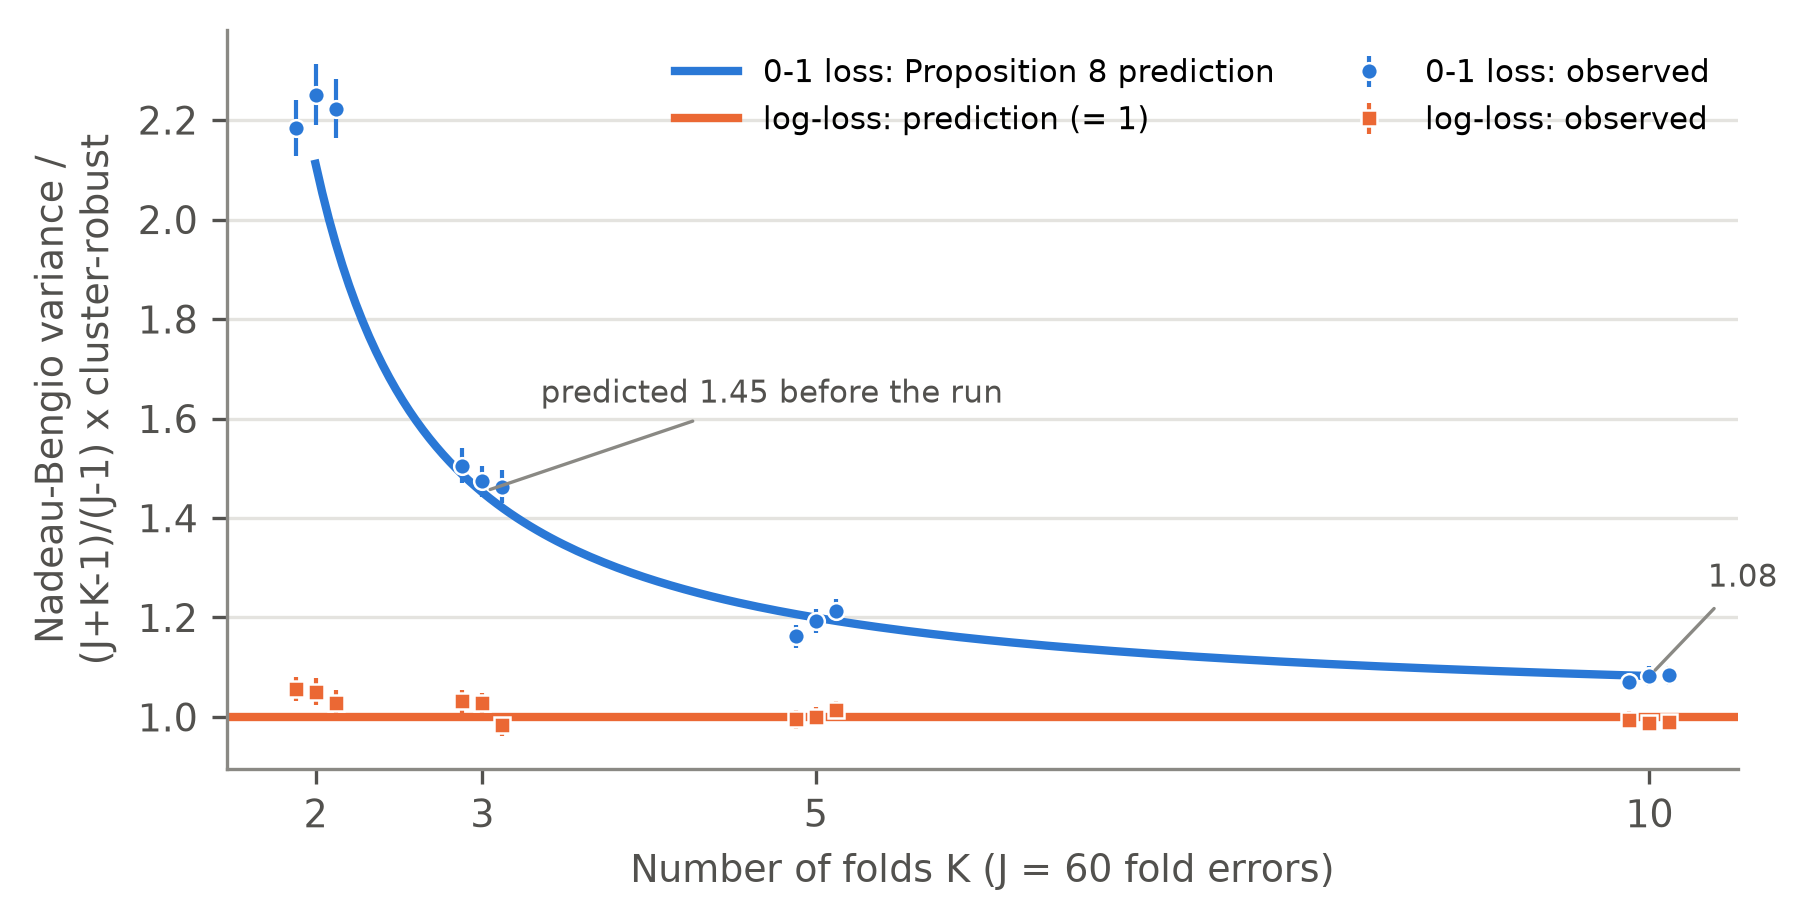
\includegraphics[width=\textwidth]{figures/paper_nb_theory.png}
\caption{Result 2 predicts how cautious the Nadeau--Bengio correction is at any number of folds. Curve: prediction
from quantities estimated at $K=5$; points: observed at 80, 160 and 320 clusters, 400 data sets each, with 95\% Monte
Carlo intervals. $K=3$ and $10$ were predicted before they ran (results/sim\_cv\_kfold\_summary.csv).}
\label{fig:nbtheory}
\end{figure}

\emph{A prediction tested in advance} (Figure~\ref{fig:nbtheory}). We estimated the inflation factor of Result~2 from runs
with five folds, then predicted it for three folds (1.452) and ten folds (1.082) before running them. The observed
values were 1.463 to 1.505 and 1.071 to 1.084. One related prediction failed at its pre-registered precision: the ratio
of the true variance to the cluster-robust variance was 0.91 to 1.17 against a target band of 0.9 to 1.1, although
its pooled value, 1.05 (90\% interval 0.98 to 1.11), is consistent with 1.

\begin{figure}[h]
\centering
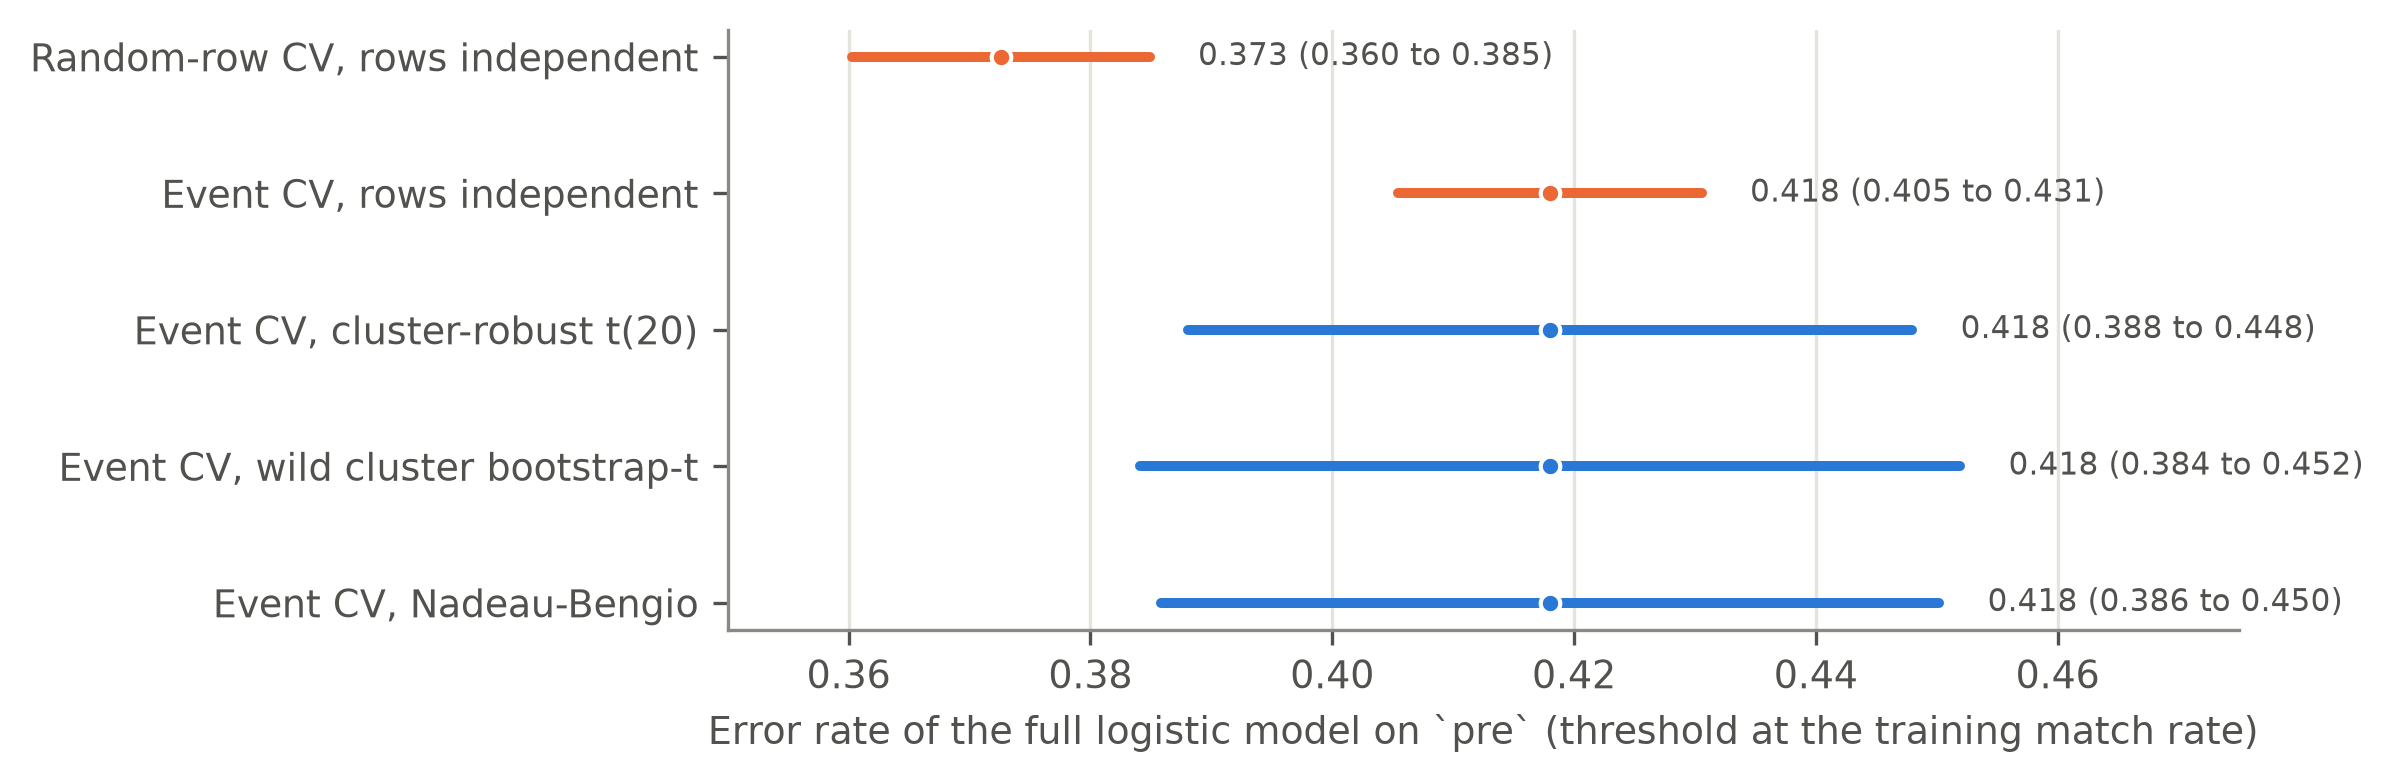
\includegraphics[width=\textwidth]{figures/paper_real_intervals.png}
\caption{On the real data, event-aware 90\% intervals for the full logistic model's error rate on \texttt{pre} are 2.4 to 2.7
times wider than the rows-independent interval, and random-row cross-validation is centred too low
(results/errorbars\_real.csv, errorbars\_final.csv).}
\label{fig:realint}
\end{figure}

\emph{On our data} (Figure~\ref{fig:realint}), the three recommended intervals agree to within 0.004 and are 2.4 to 2.7 times
as wide as the rows-independent one, and random-row cross-validation reports an error rate 0.045 lower, because it
scores people the model has already met.

\subsection{Result 3: the usual cross-validated AUC runs low when events differ}

The AUC is the fraction of (match, non-match) pairs ranked correctly (Section~\ref{sec:beyond}). The usual way to
cross-validate it, which we also used, pools the held-out predictions of all $K$ fold models and ranks all pairs
together. Pooling is known to bias the AUC downward slightly \cite{Parker:2007}, \cite[Section 2.4]{Forman:2010},
\cite[Section 3]{Airola:2011}. We found that clusters make this bias much larger, and explained why. When a match from
one fold is compared with a non-match from another, each was scored by a model that was trained on the other one's
event. The match's event tends to have had more matches than predicted, so the model trained on it, which scores the
non-match, predicts matches a little more readily and scores the non-match higher. Likewise the non-match's event
tends to have had fewer matches than predicted, so the model trained on it, which scores the match, scores the match
lower. Both effects push the pair toward the wrong order, so the pooled AUC is pulled below the AUC of any single
model. A second-order version of the argument behind Result~2 gives a formula for the size of the
bias, which shrinks in proportion to $1/G$ and does not shrink with more folds (Appendix~\ref{app:theory}). The fix is
simple: compute the AUC only over pairs whose two dyads are in the same fold but in different events.

\begin{figure}[h]
\centering
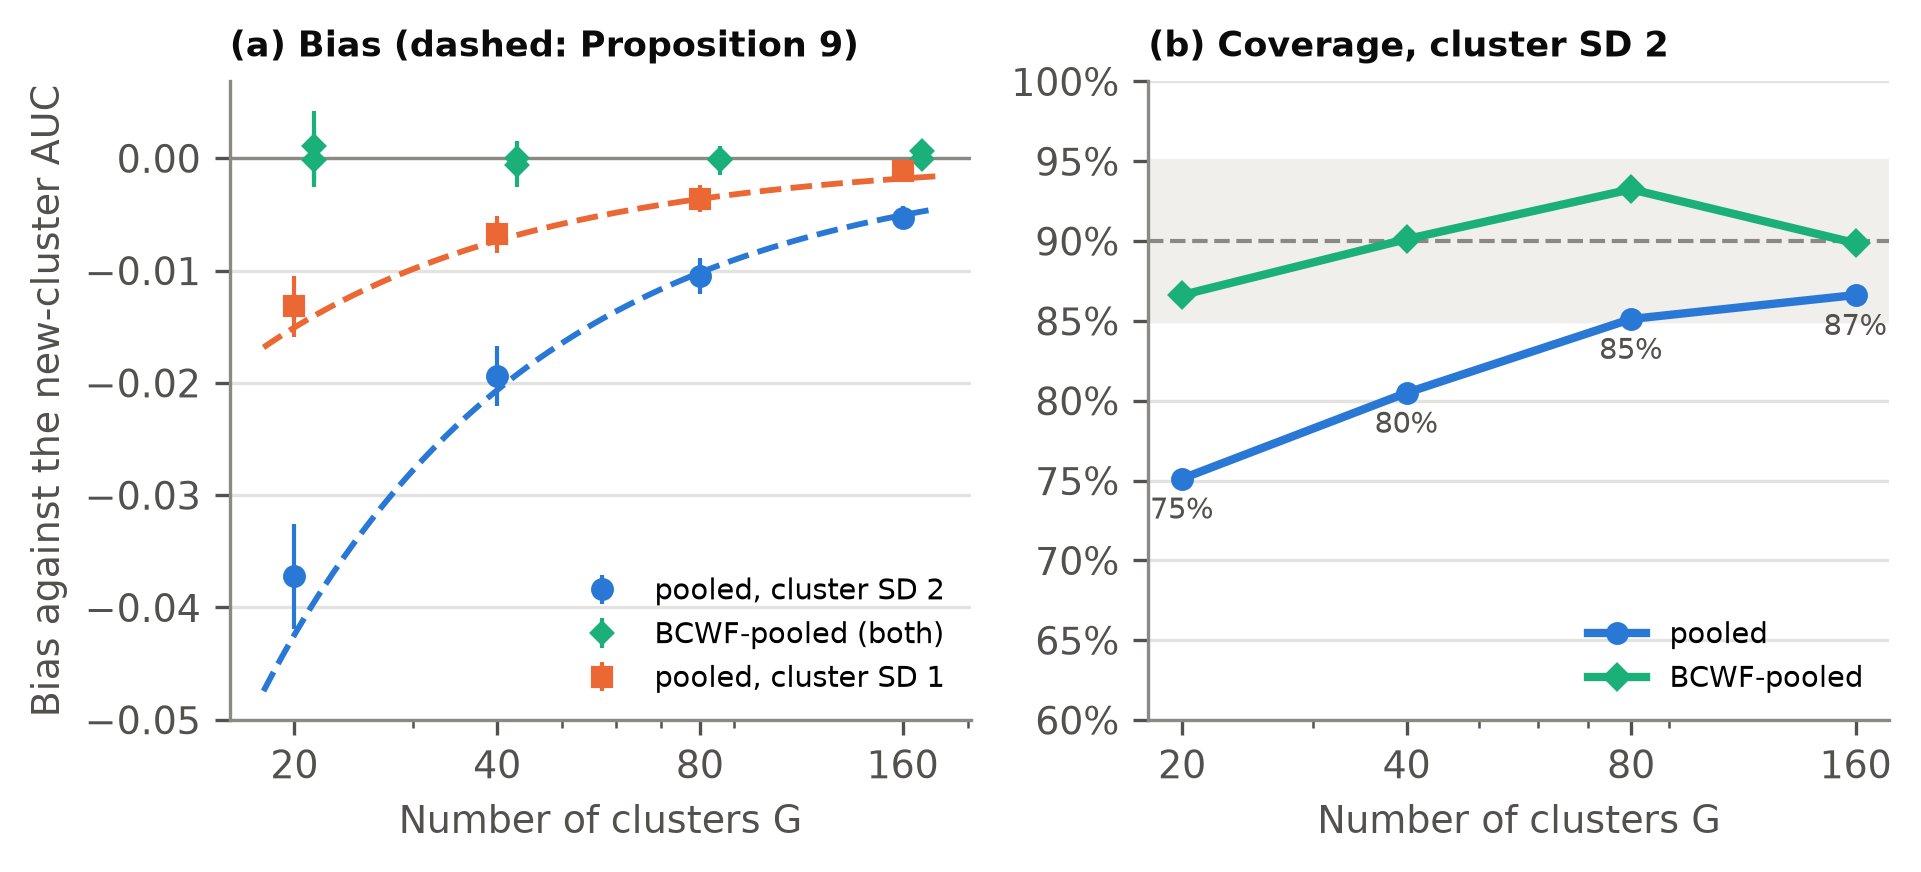
\includegraphics[width=\textwidth]{figures/paper_auc_bias.png}
\caption{Pooling held-out predictions across fold models biases the AUC downward under clustering; comparing pairs
within folds fixes it. (a) Bias against the new-event AUC, with the formula of Appendix~\ref{app:theory} dashed; (b)
coverage of 90\% intervals with strong event effects. Synthetic clusters of 40 rows, 400 data sets per point
(results/sim\_cv\_auc\_summary.csv, sim\_cv\_auc\_components.csv).}
\label{fig:aucbias}
\end{figure}

In simulation (Figure~\ref{fig:aucbias}) the pooled AUC was too low in all 12 settings with event effects, by up to
0.040, about one standard error with 20 events, and its 90\% interval covered as little as 75\%. The formula predicted
the size of the bias to within 1.3\% to 5.1\%, and with ten folds to within 1.4\%; with two folds and strong event
effects it was 18.6\% too large, so that pre-registered test failed (a larger rerun put the gap at 5.8\%). The
within-fold version was unbiased to within 0.11 standard errors and covered 89.9\% on average with 40 or more events.
On our own data the two versions agree on average (difference $-0.004$ to $+0.002$ over 20 random fold assignments),
and the formula, evaluated on our data, predicts a bias of only $-0.001$, so the AUCs in Section~5 stand.

\subsection{Recommendations}

\begin{enumerate}
\item Hold out whole events; random-row folds answer a different question (Lemma~\ref{lem:what}).
\item Use the cluster-robust standard error with $t$ quantiles on $G-1$ degrees of freedom, or the wild cluster
bootstrap when event sizes differ a lot.
\item The Nadeau--Bengio correction is safe on event folds and slightly cautious; never use it on random-row folds.
\item For the AUC, compare pairs within folds instead of pooling all predictions, when events differ in how often
people match.
\item When testing an error bar by simulation, draw new events in every simulated study.
\end{enumerate}

Most ingredients here are known: grouped cross-validation, cluster-robust standard errors, the Nadeau--Bengio
correction and the pooling bias of the AUC. What we add is how they behave together when observations come in
clusters: Result~1, the predictable caution of the Nadeau--Bengio correction in Result~2 with its test in advance, and the
explanation and size of the clustered AUC bias in Result~3. The results were checked by an adversarial review
(\texttt{proposals/09}); our mathematical lead's review is pending.
